\documentclass[chi_draft]{sigchi}

 \toappear{9th Seminar on Research Trends in Media Informatics (RTMI '17). February 2017, Ulm University, Ulm, Germany.}

% Arabic page numbers for submission.  Remove this line to eliminate
% page numbers for the camera ready copy
\pagenumbering{arabic}

% Load basic packages
\usepackage{balance}  % to better equalize the last page
%\usepackage{graphics} % for EPS, load graphicx instead 
\usepackage{graphicx}
\usepackage{tabularx}
\usepackage{enumitem}
\usepackage[labelfont={bf},textfont={bf},font=small]{caption}
\usepackage[labelfont={bf},textfont={bf},font=small]{subcaption} % if two images are rigth next to eachother
\usepackage[T1]{fontenc}
\usepackage{txfonts}
\usepackage{mathptmx}
\usepackage[pdftex]{hyperref}
\usepackage{color}
\usepackage{booktabs}
\PassOptionsToPackage{hyphens}{url}\usepackage{hyperref}
\usepackage{textcomp}
% Some optional stuff you might like/need.
\usepackage{microtype} % Improved Tracking and Kerning
\usepackage{ccicons}  % Cite your images correctly!
\usepackage[utf8]{inputenc} % for a UTF8 editor only
\usepackage{tikz}
\newcommand*\circled[1]{\tikz[baseline=(char.base)]{
            \node[shape=circle,draw,inner sep=2pt] (char) {#1};}} % circled icons for image citation
\newcommand{\divider}{
	\begin{center}
		\small
		$\ast$~$\ast$~$\ast$
	\end{center}
}
						
% If you want to use todo notes, marginpars etc. during creation of your draft document, you
% have to enable the "chi_draft" option for the document class. To do this, change the very first
% line to: "\documentclass[chi_draft]{sigchi}". You can then place todo notes by using the "\todo{...}"
% command. Make sure to disable the draft option again before submitting your final document.
\usepackage[backgroundcolor=yellow,textsize=small]{todonotes}
\usepackage{blindtext}

% Paper metadata (use plain text, for PDF inclusion and later
% re-using, if desired).  Use \emtpyauthor when submitting for review
% so you remain anonymous.
\def\authorname{Tobias Lahmann}
\def\plaintitle{Games and the Virtual Reality:\\An Introduction to Research Trends}
\def\plainauthor{\authorname}
\def\emptyauthor{}
\def\plainkeywords{Virtual reality, games, psychology, research, interaction, development}
\def\plaingeneralterms{Documentation, Standardization}

% llt: Define a global style for URLs, rather that the default one
\makeatletter
\def\url@leostyle{%
  \@ifundefined{selectfont}{
    \def\UrlFont{\sf}
  }{
    \def\UrlFont{\small\bf\ttfamily}
  }}
\makeatother
\urlstyle{leo}

% To make various LaTeX processors do the right thing with page size.
\def\pprw{8.5in}
\def\pprh{11in}
\special{papersize=\pprw,\pprh}
\setlength{\paperwidth}{\pprw}
\setlength{\paperheight}{\pprh}
\setlength{\pdfpagewidth}{\pprw}
\setlength{\pdfpageheight}{\pprh}

% Make sure hyperref comes last of your loaded packages, to give it a
% fighting chance of not being over-written, since its job is to
% redefine many LaTeX commands.
\definecolor{linkColor}{RGB}{6,125,233}
\hypersetup{%
  pdftitle={\plaintitle},
  pdfauthor={\plainauthor},
%  pdfauthor={\emptyauthor},
  pdfkeywords={\plainkeywords},
  bookmarksnumbered,
  pdfstartview={FitH},
  colorlinks,
  citecolor=black,
  filecolor=black,
  linkcolor=black,
  urlcolor=linkColor,
  breaklinks=true,
}

% End of preamble. Here it comes the document.
\begin{document}

\title{\plaintitle}

\numberofauthors{1}
\author{
	\alignauthor{\authorname\\
		\affaddr{Ulm University}\\
		\affaddr{Ulm, Germany}\\
		\email{tobias.lahmann@uni-ulm.de}}
}

\maketitle

%----------------------------------------------------------------------------------------
%	Document
%----------------------------------------------------------------------------------------

\begin{abstract}
Virtual Reality techniques are very well suited for games as they incorporate users into the action and offer great potential for developers to extend the experience conveyed in their games. Understanding the advantages but also the disadvantages of VR in all fields of gaming is important for the future advancement of the fields.
The many varying aspects and different field of needed research for \textit{Games in VR} will be examined here.
Other literature is often focusing either on the field of games and analyzing the game-impacts on players or the psychological affects of games, or is studying the field of virtual reality and the affects of this.
The objective of this publication is to combine both fields and show future development of games in virtual reality.
\end{abstract}


\keywords{\plainkeywords}

\section{Introduction}
%\todo[inline]{write introduction}

The virtual generation and perception of real environments or imaginary settings, rendered by a computer using specialized software, is referred to as virtual reality (VR). Its goal is to simulate a user's physical presence in this environment, by enabling the user to interact with this space and any objects depicted therein using specialized display screens or projectors and other devices.

The potential of virtual reality in gaming is an enormous factor both for the scientific and commercial regarding its multitude of use cases. 

In the past decade a variety of electronic devices has reached the marked and found its way into the homes of consumers. Gaming consoles have become entertainment systems offering more than just the gaming aspect. Computers gained the abilities of past supercomputers and are far more than workstations for the majority of modern population. With technological advancements made in the past 50 Years and popularity gains of these systems also the gaming industry has reached its heyday. 

VR, although expensive, gains more interest and the audience grows almost daily. 
Games that do not naturally support VR are searching for ways to include VR in their games, described in the section \textit{Games And VR}\ref{sec:gamesNvr}.

\begin{figure}%[h]
	\centering
	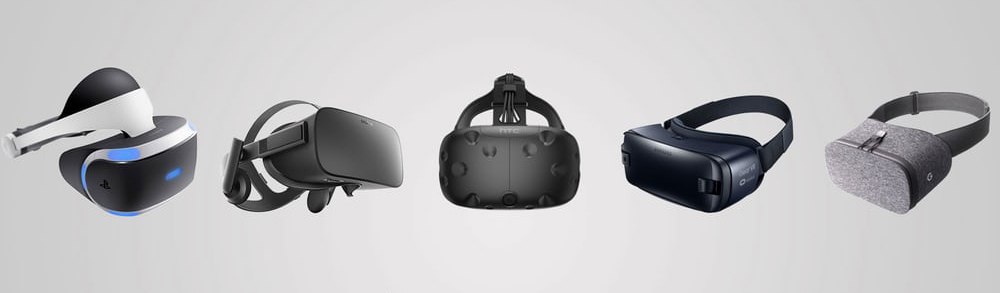
\includegraphics[width=0.99\columnwidth]{./figures/vr-hmd}
	\caption[vr-hmd]{Overview of different consumer HMD as available in late 2016. FLTR Plystation VR, Oculus Rift, HTC Vive, Samsung Gear VR, Daydream View.\footnotemark}~\label{fig:vrHMD}
\end{figure}
\footnotetext{\textcopyright~Newatlas, [Online; accessed January 04., 2017],[Digitally revised] \url{http://img-2.newatlas.com/vr-comparison-2016-b-2.jpg}}

The development of consumer friendly head mounted devices (HMD) for VR, as to see in \textbf{Figure~\ref{fig:vrHMD}}, has just picked up in recent years with systems like the \textit{Oculus Rift in March 2016}, the \textit{HTC Vive in April 2016}, the \textit{Samsung Gear VR in August 2015}, the \textit{Playstation VR in October 2015} or the \textit{Daydream View in November 2015}. 

Many developers have already started to develop games that use the advances of VR and are serving quick, but the research on this fields has lacked behind on reliable results regarding the ideal approach to points such as immersion, interaction and performance. This publication intends to show the many disciplines and what research can be done to improve VR in Games.



\section{Games and the Virtual Reality}
\label{sec:gamesNvr}

To catch a brief insight into games that both support playing with or without HMD and to further introduce research aspects of the following section this paragraph is intended to list a few differences, similarities and uniqueness within games. An overview of these games can be found in Table~\ref{tab:popularGames}, where some properties of them are listed. 

Starting with \textit{Minecraft}~\cite{game:minecraft}. an open world sandbox game where the player controls his playable character by navigating with the keyboard or game controller. The goal is to mine blocks of different material and craft them into objects which he will need to complete the game. As it is an open world game the player can move to different areas in order to gather some items needed~\cite{game:minecraft}. \newline
A disadvantage of this game in VR is the locomotion method needed in order to move around the world. Since the game has not many stationary tasks and it depends on the ability of the user to move around it holds greater potential for the virtual reality sickness (Explanation see Section \textit{Further Research Trends: Increasing The Performance Of Devices For VR Gaming}) occurring.

Another game is \textit{Keep Talking and Nobody Explodes}~\cite{game:keepTalking} a puzzle game where one player has to describe and disarm a virtual explosive charge in a given time. His team members, who cannot see the bomb, have to explain what he has to do in order to disarm the bomb and to save his and the team members lives~\cite{game:keepTalking}. The game mechanics are different from those of Minecraft. The player wearing the HMD has a stationary task and just needs to interact with objects in his direct vicinity. \newline
Because of this only natural locomotion the peril of becoming sick is very weakly present.

\begin{figure}
	\centering
	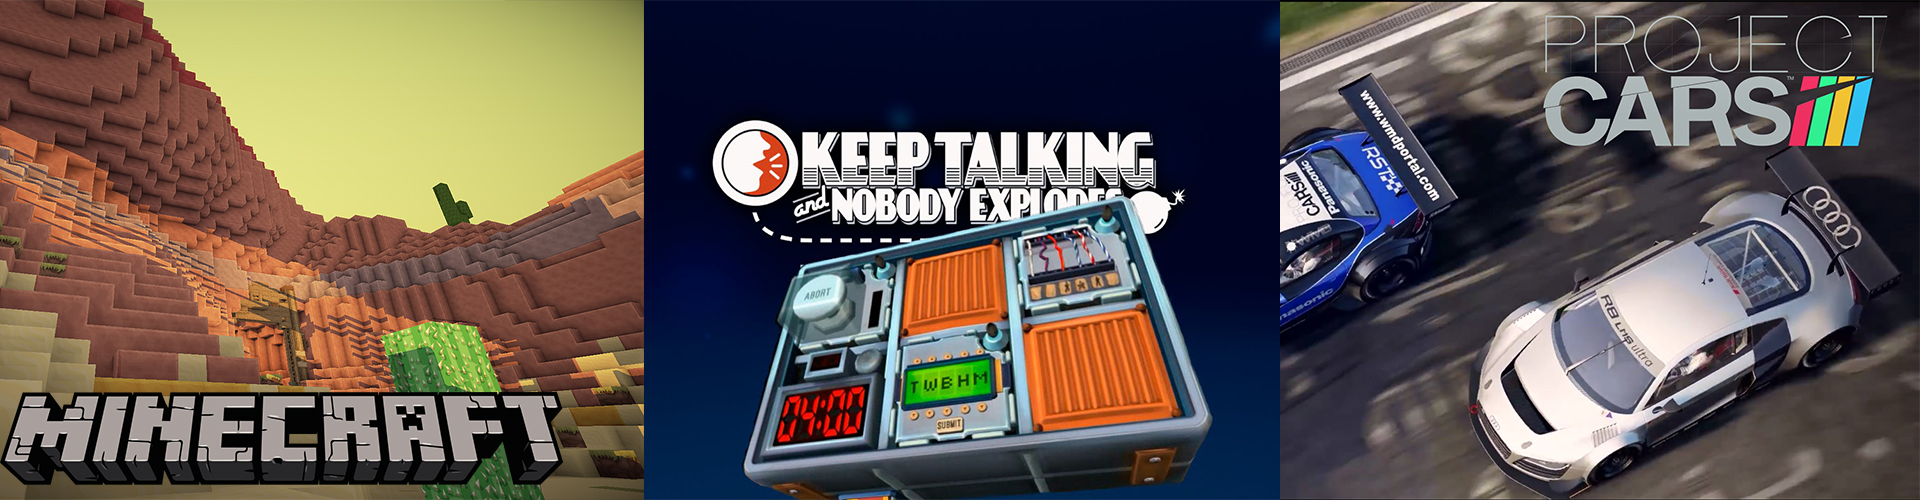
\includegraphics[width=0.99\columnwidth]{./figures/banner}
	\caption[banner]{The three presented games. FLTR Minecraft, Keep talking and nobody explodes and Project CARS. Each game offers native VR Support on multiple devices and has different interaction methods for locomotion. Image source in footnote 1 \textcolor{white}{\footnotemark[1]}}~\label{fig:banner}
\end{figure}
\footnotetext[1]{
	\textcopyright~Mohjang, Steel Crate Games, Slightly Mad Studios, [Online; accessed January 04., 2017],[Digitally edited] \url{https://pixabay.com/p-354458} \url{https://i.ytimg.com/vi/Apwa_ksMvM0/maxresdefault.jpg} \url{https://i.ytimg.com/vi/RggvBJ2ANWo/maxresdefault.jpg} \ccbyncsa
} 
\textit{Project CARS} is a racing simulation for Microsoft Windows, PlayStation 4, and Xbox One~\cite{game:projectC}. It offers standard racing simulation whilst offering HMD based gameplay as well as normal gameplay using a monitor. The game depends on content created by its users to extend the gaming experience~\cite{game:projectC}. \newline
The locomotion is solely a cockpit locomotion, meaning that the player is sitting in a virtual car and steering with different interfaces. Because of the visual stimuli of moving inside a car but neither the vibration nor the acceleration is palpable the user could be more weakly prone to becoming VR sick.

In VR these games offer an immersive way to include the gamer into the game. Because of the different approaches to solving problems of VR more static games like \textit{Keep Talking and Nobody Explodes} and \textit{Project CARS} could have greater potential in becoming very popular in the VR gaming community. 

\begin{table}
	\caption{Popular games played in late 2016. The games offer a regular play mode, using the monitor, and a VR play mode with both the Oculus Rift and the HTC Vive. Types of Locomotion (LM): Natural Locomotion (NLM), Cockpit Locomotion (CLM), Artificial Locomotion (ALM). RPG: Role-Playing Game}~\label{tab:popularGames}
	
	\renewcommand{\arraystretch}{1.3}% for the vertical padding
	\begin{tabular*}{\columnwidth}{ p{33mm} l r l }
		Gametitle & Genre & \parbox[c][2.2em][t]{2cm}{\begin{flushright}$\dfrac{Players}{Month}$(\footnotemark[2])\end{flushright}} & LM \\
		\hline
		Minecraft & RPG & 990 K & ALM \\
		Keep Talking and \newline Nobody Explodes & Puzzle & 153.3 & NLM \\
		Project CARS & Racing & 1.01 K & CLM\\
	\end{tabular*}
	
\end{table}

\footnotetext[2]{\url{http://steamcharts.com}, accessed Jan. 3., 2017}

\subsection{Popularity Of VR Games}
Since the beginning of game development and virtual reality in the 20th century there has been a huge potential to include the user in a virtual environment. Some systems have been developed in the past five years that simplify some processes of work for different disciplines. 

Games have just lately adopted the potential for this immersive form of gaming. VR offers new dimensions of freedom to include the player into a game world and to tell stunning stories.

Using a virtual environment to show worlds to players has the great advantage of giving them the feeling of being in the middle of the event, but the game has very limited possibilities to tell stories with much variety. This is that the game can not change perspectives as easy. 

While games that do not use VR can handle attention themselves by just moving the camera, VR is bound to the camera perspective of the gamer. These games can show views from other perspectives without worrying about the user becoming confused. VR games need another way to handle interactiveness, the user has to hold some kind of controller interface to tell the system what he wants to do. Games outside of VR have similar interface problems but the process has been researched more than the interaction with VR games. Simultaneously VR games require a much more active way of interaction, because the user has to complete physical tasks as he is playing the game. This can be a negative point for people who would just rather enjoy a game than have a minor workout while playing.

It is not yet set whether the implementation of VR into the three games from above has increased the popularity drastically. Official values regarding players and other statistics are hard to acquire. Certainly the game developers have not had losses in terms of player count after implementing VR support since the games are popular for regular players already. \newline
Virtual reality offers a broad new way of experiencing games. Why is it that the virtual reality has not yet reached a higher popularity with a wide range of players?

\divider

In January 2017 I have created an online survey asking players and non players alike on their opinion regarding virtual reality and games. Withing the 5 days of activity of the survey almost 50 participants had taken part in it. Although I have only scratched the surface of the topic with this number of participants a very good overview of different gaming generations can be given. The age spanned from 12 to 50 years. While most participants came from northern America also a significant amount came from Europe and a very minor amount from Asia and Oceania. \newline
The survey showed that a majority of people had never played a virtual reality game before. When asked why the most common answer was regarding the pricing of VR systems in general. Some people answered that they did not have enough space in their living room and others said they where not satisfied with the quality and development of VR as of today. This opens up another question that researchers have to tackle: is VR gaming a luxury good reserved for only a few? \newline
It was further found that most persons describing themselves as gamers would agree that VR games should be immersive and intuitive. The results can be seen in Table \ref{tab:study} as well as Figure \ref*{fig:study}. Intuitive meaning that the interaction and locomotion in the game is as close as possible to movement in the real world. Most participants agreed that VR do not have to be simple regarding interaction and problems presented. \newline 
The study has lastly shown that most of the people that have tried a VR game in person would describe themselves as gamers, although also many other participants affirmed this question.\newline The last question resulting is if people are more likely to test VR in person if they think they already are gamers or if VR games can reach a broader audience in the future due to the higher approachability of games. Every person knows how to pull a virtual bow since it is close to real world interaction rather than interacting with other interfaces. 

\begin{table}[h]
	\caption{Gamers and non games have been asked to rate the following aspects, whereas 1 means they strongly disagree, 4 means they strongly agree - 0: unsure. The question asked was whether they thing a VR game should be...}~\label{tab:study}
	
	\renewcommand{\arraystretch}{1.3}% for the vertical padding
	\begin{tabular*}{0.98\columnwidth}{ p{28mm} | @{\extracolsep{\stretch{1}}}*{5}{r}@{}}
		 & 1 & 2 & 3 & 4 & 0 \\
		\hline
		Immersive & 0 & 0 & 10 & 37 & 2 \\
		Active & 2 & 11 & 23 & 11 & 2 \\
		Intuitive & 0 & 2 & 24 & 19 & 4 \\
		Simple & 5 & 25 & 10 & 4 & 5 \\
	\end{tabular*}
	
\end{table}

\begin{figure}[h]
	\centering
	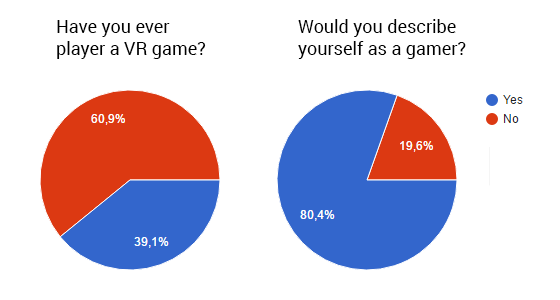
\includegraphics[width=0.90\columnwidth]{./figures/study}
	\caption[study]{Most of the people asked have not tried any VR games yet. Also most of the participants would say they are gamers.}~\label{fig:study}
\end{figure}

\subsection{Motivation In Games}

The staff of \textit{Quantic Foundry}~\cite{online:motivation}  have developed an online survey for categorizing 
gamers and their motivation.
Users can receive a personalized report on their gaming incentive by completing a survey with about 14 questions on their approach towards games, their different gaming aspects and habits. \newline
Over the course of early 2016 until late august 220 thousand individual people took the test. Among the participants were about 81\% male and 18\% female users. The age ranged from 13 to 77 years and the median was 25 years. Most of the gamers came from North America and the western EU.

The most interesting part is the model that emerged from the data they have got. The categories can be seen in Figure~\ref{fig:gameMotivation}. They have described the categories as follows:

\begin{figure}
	\centering
	\begin{subfigure}[b]{0.49\columnwidth}
		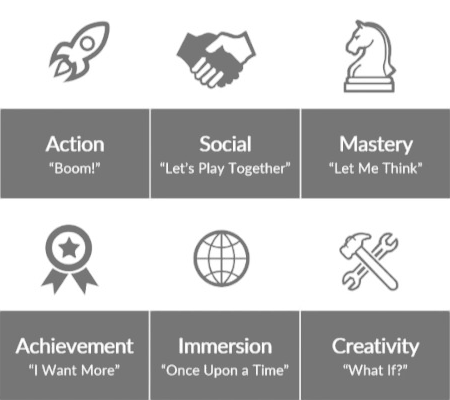
\includegraphics[width=\textwidth]{./figures/motivation}
		\caption[motivation]{Categories of motivation}~\label{fig:gameMotivation}
	\end{subfigure}
	\begin{subfigure}[b]{0.49\columnwidth}
		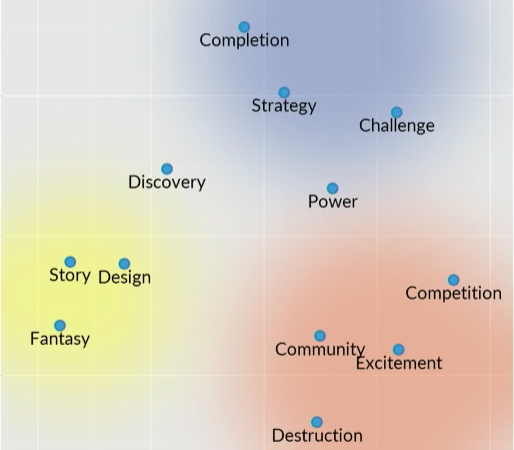
\includegraphics[width=\textwidth]{./figures/clusters}
		\caption[motivation]{Motivational clusters}~\label{fig:motivationClusters}
	\end{subfigure}
	\caption[]{Left: The 6 categories of motivation in games as described by Nick Yee of \textit{Quantic Foundry} in their talk about motivation. | Right: Three motivational clusters that followed from the study of Nick Yee and \textit{Quantic Foundry}. Blue is mastery-achievement cluster, yellow is immersion-creativity cluster and red is action-social cluster. Image source in footnote 3\textcolor{white}{\footnotemark[3]}}
\end{figure}

\footnotetext[3]{"Gamer Motivation Profile Findings - \#GamesUR US Conference 2016" Quantic Foundry Website, March, 25., 2015, accessed November 05., 2016, \url{http://quanticfoundry.com/2016/04/07/gdc-talk/}}

\begin{description}
	\item[Action] \textit{''The appeal of mayhem and chaos and exciting, fast paced game play context.''}~\cite{online:motivation} \newline Action as motivation addresses people who like the thrill and the challenge.
	
	\item[Social] \textit{''Contains both: the challenge and the interesting collaboration and socializing.''}~\cite{online:motivation} \newline The social category describes people who like to socialize, help and/or compete with others.
	
	\item[Mastery] \textit{''Is about long term planning and thinking. Practicing the game to take on the highest difficulty or the enjoyment of strategy.''}~\cite{online:motivation} \newline It mostly appeals to the peoples wish to make complex decisions.
	
	\item[Achievement] \textit{''Different ways of getting points in the context of the game. Credits, points, stars, trophies et cetera. Also, in another way, power. Meaning leveling up or getting the best equipment and gear.''}~\cite{online:motivation} \newline Rouses some peoples collector's passion as well as appeals to people who want to feel powerful.
	
	\item[Immersion] \textit{''Different ways of becoming embedded in the story of the world.''}~\cite{online:motivation} \newline For those people who want to become someone else or want to experienced interesting stories.
	
	\item[Creativity] \textit{''Making the game your own in any kind of way. [...] Uniqueness, customization and discovery.''}~\cite{online:motivation} \newline Mostly describing people who like creativity in games and those who want to customize their experience.

\end{description}

It was found that those gamers that fit into one of the six main categories often prefer similar aspects of a game as that players falling into another of the categories. \newline
From this categorization the next step for them was to analyze their results. They have found that at a high level there are \textit{three} motivational clusters that combine multiple of the categories into sections of similar gaming behaviors. \newline 
These clusters can be seen in Figure~\ref{fig:motivationClusters} and are described as follows:

First there is the \textbf{action-social} cluster, combining the action-packed gameplay with social activities in games. As described before this cluster holds people that like the thrill of the game and want to have action, but it also contains the challenge of the game as well as socializing. It was found that these gamers share some common interests such as \textit{community}, \textit{destruction} and \textit{excitement}. \newline
The second cluster is \textbf{mastery-achievement}, containing players that want to become better. It is standing to reason that these classes are very much correlating in many ways. A multitude of games today offer many ways of collecting items as part of achievements and are also awarding them for collected rare items. A more fine grained description of the people in this category would be to describe them as gamers who like points such as \textit{competition}, \textit{strategy} and \textit{challenge}. \newline
And the last cluster is \textbf{immersion-creativity}. With points like \textit{story}, \textit{fantasy} and \textit{design} it is the most compact in its variance. It does not surprise that immersion correlates with creativity as they are already very similar in many ways. 

They have further found that there are two traits which form kind of like bridges between clusters. \newline
For one that is \textit{discovery}, where the player wants to discover new ways of playing the game as well as discover exciting places inside of the in game world. This can be categorizes both in the \textit{mastery-achievement} and the \textit{immersion-creativity} cluster because it holds aspects from the first as well as the latter.\newline 
The second is indicated as \textit{power}, spanning a bridge between \textit{action-social} and \textit{mastery-achievement}, and appeals to the user to satisfy the urge to master the game and also be in the center of action. 

\divider

In virtual reality not all categories convey easily. While \textit{action}, \textit{immersion} and \textit{creativity} are often already well implemented in todays games missing research on the \textit{social}, \textit{achievement} and \textit{mastery} parts avert a pivotal statement on the subject. \newline
VR games are frequently designed to imply action. Many games use fast-paced gameplay techniques to offer the player thrilling experiences. This arises from the fact that modern HMDs provide not enough comfort to keep playing for very long periods of time. Games therefor have to entertain the user fast and convincing. Also they often require creative problem solving skills of their users and offer great ways of designing or customizing the game.\newline
The immersion is already given by the fact that the user is playing a VR game, so this will not be specified further. 

On the other hand not many approaches have been made to include other real players into the game. With this the social aspect of gaming motivation lacks somewhere behind other categories. A very small fraction of games have a well developed idea of how to include a second player into the game and even less games have a perfect representation of another player in the game, i.e. via avatar. \newline
Gamers can not interact with other people very well while playing VR games, this not only owed to the fact that VR can not yet represent other players well, but also due to the missing presence of items in the real world. An application for real world items is that in games for most social interaction a player can 'trade' items easily. How this problem could be tackled will be discussed in the section \textbf{Further Research Trends}. \newline 
The other two categories have not been developed into VR games a broad as in other games it remains uncertain what will be in the future.

With the previously presented games come different motivational inducements. \newline
In Minecraft, the most frequently played game of the three, motivation will most certainly fall under the creativity point when playing on PC or console without HMDs. Whereas using a VR headset to play it will most likely address immersion at least as much as creativity because the game world and interaction will become more convincing to the user. Hence Minecraft clearly belongs to the \textit{immersion-creativity} cluster both in normal play mode as well as using a HMD.

Keep Talking and Nobody Explodes has already a very immersive approach to playing the game. The view of the player does not differ much from the point of view gained in a the virtual environment, although the user can be even more included when playing with a HMD.

Project CARS recieves more immersiveness as well as a better feeling for the action in the game since it varies much from the gameplay without headset. 

In conclusion, the motivation of all three games gets included or increases in the \textit{immersion} category when using HMDs. The game developers have to implement a well defined method of interaction and a clear way of transferring the feeling inside their games to develop good VR games. 

\subsection{Existing Locomotion Techniques}
\label{sec:exLocomotion}

There are three basic categories of locomotion present at this time in VR: 
\textbf{artificial}, \textbf{natural} and \textbf{cockpit locomotion} as of the Wikipedia article on VR games with Oculus Rift support \cite{wiki:vrOculus}.

The principle described as \textit{artificial locomotion} is the method of 
moving in the virtual environment by triggering interfaces and telling the game 
where the player wants to go. This method is often used because it offers a great 
degree of freedom. But it also has the greatest disadvantage because the users' 
senses provide different signals to the brain and thus holds the greatest 
potential to cause motion sickness.

There are different specific methods of artificial locomotion:
\begin{description}
	\item[Interface movement]By using the provided interface devices the user 
	can steer the virtual representation of himself in different directions. 
	Depending on the game it has up to three dimensions of motion and thus 
	degrees of freedom.
	\item[Point and teleport]The user has to point, using his provided input 
	method on a surface and confirm the selection. The 
	game then moves the camera, the virtual representation of the player, to the 
	location. By using this method the user can move through a world without 
	the need to actual physical change of location. An advantage is that 
	the user can observe at worlds from different points of view.
\end{description}

In \textit{natural locomotion} only the motion and rotation of the users head is used. It requires no movement indicated through an input interface. This interaction method with the game worlds is very static and thus these kind of games do not cause sickness and enable constant mental presence and longer playtimes to the user.

With natural locomotion the user is limited to a local position in the game as well as the virtual environment. But there are also different approaches to making games using this type of locomotion:
\begin{description}
	\item[Interaction with objects]The user can interact with objects right in 
	front and around him. The objects are movable, turnable and sometimes 
	scalable by using the game interfaces.
	\item[Moving the view around the main game object]Inside the game the user can 
	specify from what angle he wants to look at the game objects in focus. 
	Again by using the game interface he can position the camera and with that 
	the position from which he is interacting with the object.
\end{description}

\textit{Cockpit locomotion} in games use a vehicle with a cockpit or stationary interaction space in a movable item to let the player traverse a large environment. Whether this evokes virtual reality sickness varies between persons, the size of the cockpit, and the intensity of the maneuvers that are performed. Generally, users are less likely getting sick if only gentle movements are done.

In cockpit locomotion the movement of the camera is not possible without moving 
the nearby surrounding environment
\begin{description}
	\item[Cockpit]With a near vicinity of objects displaying a cockpit, such as 
	the one of an airplane, a car or comparable vehicles the user can move 
	himself and his surrounding around the virtual game world and with this 
	move from one place to another.
	\item[Stationary Items]Meaning surroundings that are not movable. In this 
	locomotion technique only the orientation of the device the user is using 
	can be changed. This can be adapted to stationary weaponry or other 
	stationary items.
\end{description}

In research are not many approaches to the pros and cons of these different locomotion 
techniques and no clear statement can be given on the best solution. 
Future research trends will be looked at in the following section under 
\textit{Locomotion}.


\section{Further Research Trends}

This section is not intended to describe every aspect to its fullest, but to illustrate a showcase of possible and/or desirable developments of VR and HMD in the very near future. \newline
Some mentioned technologies are only predictions and time will show which of these can become a reality in the next couple of years. \newline
Since the leading edge of virtual reality will be computer generated VR for a long time to come these predictions will refer mostly to this~\cite{online:oculusKeynote}. The innovations will find its way into mobile and console VR over time, but the power, compute and pricing advantages will mean that computer generated virtual environments will provide the most complex and convincing experience for a very long time.

\subsection{Improvements For VR Games}
\subsubsection{Locomotion}
\label{sec:locomotion}

\begin{figure}
	\centering
	\begin{subfigure}[b]{0.38\columnwidth}
		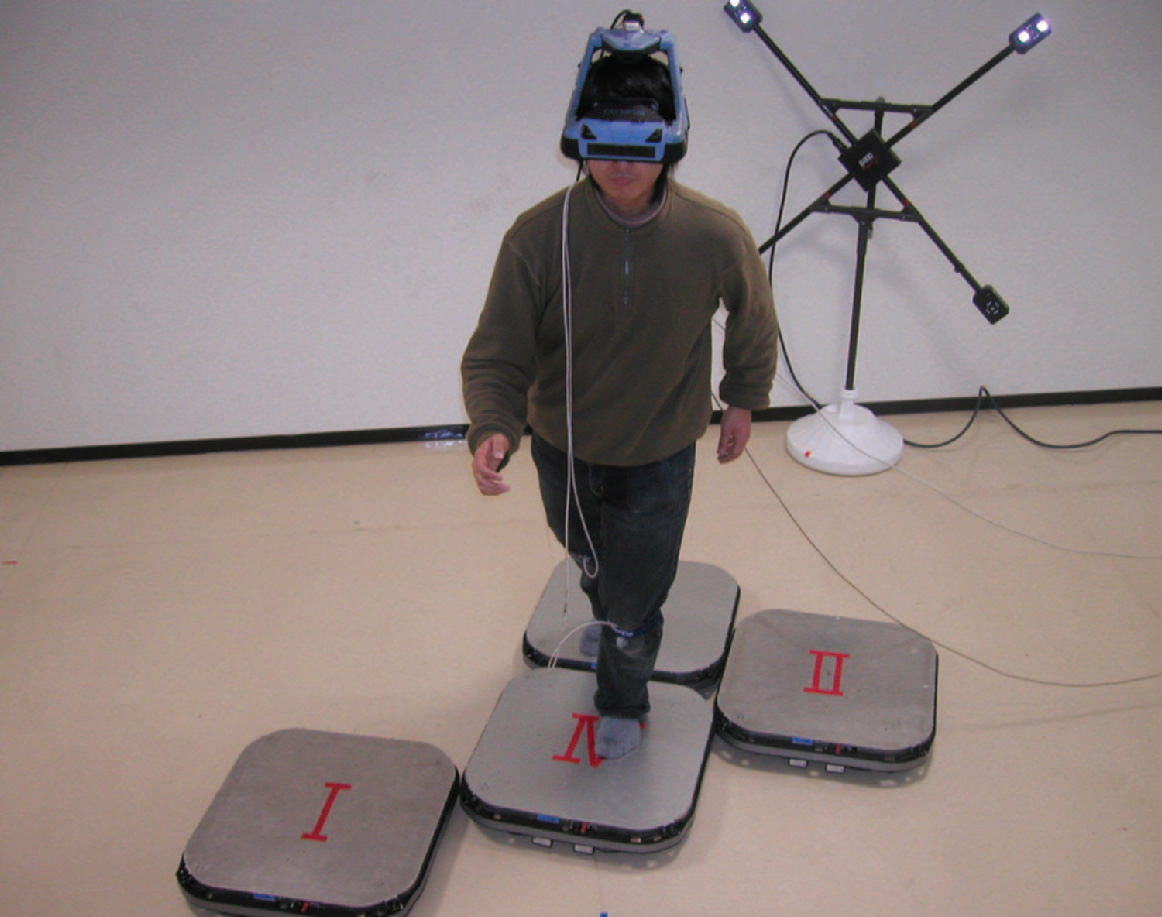
\includegraphics[width=\textwidth]{./figures/01381227}
		\caption{CirculaFloor\newline}~\label{fig:cirFloor}
	\end{subfigure}
	\begin{subfigure}[b]{0.38\columnwidth}
		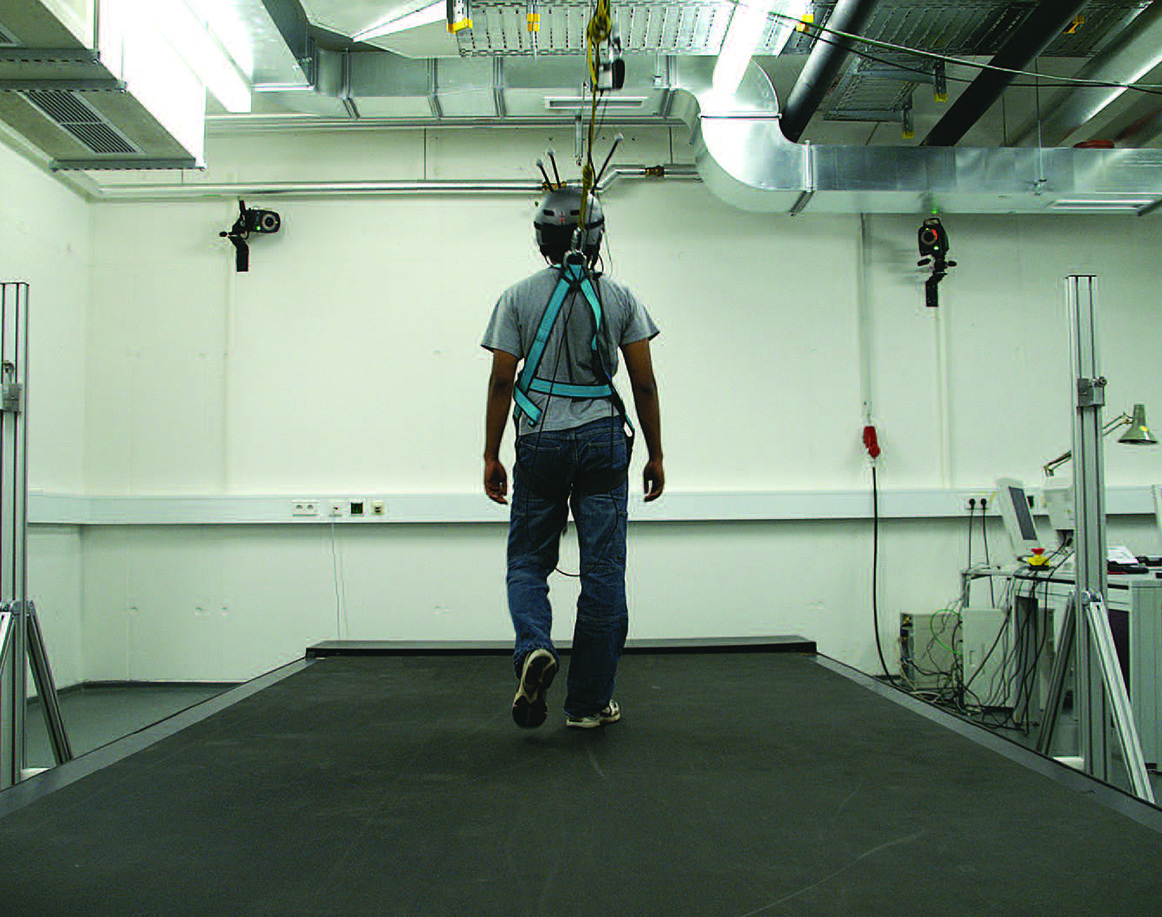
\includegraphics[width=\textwidth]{./figures/ACM_TAP_2010}
		\caption{Omnidirectional treadmills}~\label{fig:omniTread}
	\end{subfigure}
	\begin{subfigure}[b]{0.21\columnwidth}
		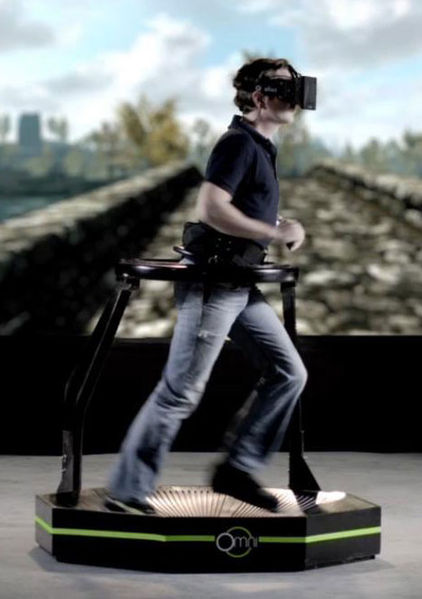
\includegraphics[width=\textwidth]{./figures/422px-Virtuix_Omni_Skyrim_(cropped)}
		\caption{Omni Gaming Treadmill}~\label{fig:virtuixOmni}
	\end{subfigure}
	\caption[]{Left: The CirculaFloor using movable floor tiles to simulate a larger traversable area. | Middle: The omnidirectional treadmill used for the development of the algorithm used by Souman et. al. | Right: The Omni Gaming Treadmil from Virtuix developed to simulate large play areas for gaming. Image source in footnote 4\textcolor{white}{\footnotemark[4]}}
\end{figure}

\footnotetext[4]{~Figure~\ref{fig:cirFloor}: CirculaFloor~\cite{Iwata:2005:CLI:1078037.1079777}, Iwata et. al. | Figure~\ref{fig:omniTread}: Making Virtual Walking Real~\cite{Souman:2010:MVW:1670671.1670675}, Souman et. al. | Figure~\ref{fig:virtuixOmni}: Omni Gaming Treadmill \url{https://upload.wikimedia.org/wikipedia/commons/f/fd/Virtuix_Omni_Skyrim_(cropped).jpg}~\ccbysa}

Existing locomotion techniques have huge advantages but also disadvantages regarding immersion, simplicity and health aspects. It is a very comprehensive field of studies and research to optimize the illusion provided by a virtual environment by using better approaches towards the transition of the in game character.\newline
To enable the player to move freely inside the virtual environment different devices and techniques have been developed to offer artificial locomotion to the user. The main goal is to create a space where the user can move freely in all 3 axes at best and therefore gain an ideal gaming experience.\newline
The following approaches have been made by researchers to enable the player to move around in the in game world without the need of a large area designed like the game itself. These will be categorized under \textit{artificial locomotion} where the device described display another interface for the user to interact with, but will bypass the problems of this interaction method since the users senses receive a more persuasive feeling of movement.
\begin{description}
	\item[CirculaFloor] Approaches like the one taken by Hiroo Iwata, Hiroaki Yano, Hiroyuki Fukushima in their CirculaFloor~\cite{Iwata:2005:CLI:1078037.1079777} as seen in Figure~\ref{fig:cirFloor} have shown that shape changing interfaces are generally not hard to build. It was aimed to design a new hardware architecture that would be easy to upgrade the actuation mechanism or add new mechanisms for the creation of uneven surfaces. To achieve these goals, a configuration for a locomotion interface using a set of omnidirectional	movable tiles was designed~\cite{Iwata:2005:CLI:1078037.1079777}. \newline Each tile is equipped with a holonomic mechanism that achieves omnidirectional motion. An infinite surface is simulated by the circulation of the movable tiles. Position sensors measure the motion of the feet. The tile moves in the opposite direction of the walker’s measured direction, canceling the motion of the step~\cite{Iwata:2005:CLI:1078037.1079777}. This computer-controlled motion of the tiles fixes the walker’s position. The circulation of the tiles can cancel the walker’s displacement in an arbitrary direction. Thus, the walker can freely change direction while walking~\cite{Iwata:2005:CLI:1078037.1079777}. 
	
	\item[Omnidirectional Treadmill Algorithm]Another approach made by Souman et. al.~\cite{Souman:2010:MVW:1670671.1670675} shows the potential for omnidirectional treadmills. They developed an algorithm to steer the speed of a treadmill in such a way that VR immersiveness is not disrupted by changes in treadmill velocity. "This algorithm was developed to work with an omnidirectional treadmill ...", as shown in Figure~\ref{fig:omniTread}, "... allowing for changes in both walking speed and direction"~\cite{Souman:2010:MVW:1670671.1670675}. "A user can therefore walk in place and the VR system defines the world around him as endless space".~\cite{Souman:2010:MVW:1670671.1670675}\newline This approach tackles problems better than the CirculaFloor because it generates less disturbance in the users walking pace.
	
	\item[Omni Gaming Treadmill] Is an omnidirectional treadmill being developed by \textit{Virtuix}. Their \textit{Omni Gaming Treadmill~\textcopyright} can be seen in Figure~\ref{fig:virtuixOmni}. The Omni uses a concave, low-friction platform that enables a smooth gait and immersive walking and running motion.~\cite{online:omni}
\end{description}

Usable research to \textit{cockpit} and \textit{natural locomotion} have not yet sufficiently been made or could not been found in a satisfactory manner. The approaches towards these locomotion techniques remain a broad field of study for further research. 

In todays VR games 'virtual walls' are a widely seen solution to prevent people from walking into physical items like furniture, walls, stairs et cetera. It is interesting to notice that this is important because VR is not yet ready to support full shape recognition of objects in the living room. With this the HMD could detect hazardous situations or items and the game could substitute it as something the user might not want to touch. The experience provided by this would be more seamless.\newline
Shape recognition could also be important to develop to actively steer the users attention into directions that are open and save for the user to walk towards. On the downside the base station of the VR system must have an enormous amount of computational power to make these kind of calculations.

Useful approaches could be the research known as 'redirected walking', where the user perceives a straight line of walking in game where he is walking in a curved line in real life~\cite{razzaque2001redirected}. The game conveys the impression of a linear forward motion and utilizes a limited amount of space in this manner.

\subsubsection{Sight}

Head mounted displays of today have far less pixel density, a narrower field of view (FOV) and the lenses used have no actual method of actively focusing what the user is looking at~\cite{online:oculusKeynote}.\newline
It is important to understand that a result of human evolution is that the visual perception ot things affects the impression we get of something in an enormous way. \newline
To improve the visual representation and the image transmitted by HMDs the work on pixel density together with field of view will be standing in focus on future research iterations. It has mainly two approaches which accompanies an interesting trade-off in the usage of the resulting display resolution. Pixel density is a function of both, display resolution and field of view. One can have a higher pixel density image with a narrower field of view, or a wider field of view with a lower pixel density image~\cite{online:oculusKeynote}. \newline
It all depends on what FOV is achievable and how compelling a wider FOV turns out to be.

The two approaches are to either achieve a generally higher pixel density and with that a higher resolution on the displays or to teach the system to recognize the field of focus of the user.

A wider field of view with higher resolution will require a breakthrough in optics. Todays available lenses have a limited field of view without noticeable distortion, so new optics technology will be required~\cite{online:oculusKeynote}. This is not limited to newer or more advanced lenses but also so self adapting settings regarding distance, orientation and yaw of these. 

The used lenses of HMDs have also a fixed focus and while the human eye can adapt to different distances between objects the lenses of today stay focused around a distance of two meters~\cite{online:oculusKeynote}. This would require an entirely new lens technology synthesizing on technologies like varifocal glasses, but adapting to the position the user is looking at.

The last point can be addressed with research field like \textit{holographic displays}, \textit{light field displays}, \textit{multifocal displays} or \textit{varifocal displays} and todays research teams are already on the subject~\cite{online:oculusKeynote}.

\subsubsection{Touch}

Touching something in VR and receiving real feedback from an in game object can expand the illusion of a real virtual environment. \newline
Using some similar technology to the iDummy~\cite{online:idummy} developed by Chan et. al. developers can create various objects of different size and shape. A user wearing a VR Headset could see a specific object and feel it as if it was the real thing. Using the technology developers can extend the realm of VR to one more dimension. Together with the technology of Mahdi Azmandian et. al. in their paper \textit{Haptic Retargeting: Dynamic Repurposing of	Passive Haptics for Enhanced Virtual Reality Experiences}~\cite{Azmandian:2016:HRD:2858036.2858226} the technology could be even further expanded to having a multitude ob objects of different shapes, size and orientation in ones direct vicinity. This could enable developers to enter unknown territory of unforeseen possibilities. 

The iDummy is a mannequin technology where different body parts can be modified by using multiple servo motors. The mannequin can change its chest circumference as well as hip measurement or the width of the waist to adapt to the needs of apparel designers and represent every body shape imaginable. \newline
Haptic retargeting is the process of making the user think he is touching different objects by differentiation between them in virtual space~\cite{Azmandian:2016:HRD:2858036.2858226}. In reality these objects might be the same. 

Adapting these principles to basic shapes, like cubes, balls or tetrahedrons a very haptic way of interacting with in game objects can be pursued. A user wearing a HMD can actually touch an object, feel its presence and the device is adding a visual abstraction casuing the user to belive what he is touching is real. The player could with this method touch a ball of moderate size and see a basketball in the virtual representation of this.

Comparable research has been done on shape changing interfaces, in example by Rasmussen et. al.~\cite{Rasmussen:2012:SIR:2207676.2207781}. They define 8 types of change for objects in 2 categories:

\begin{description}
	\item[Topologically equivalent] Change of \textit{orientation}, \textit{form},  \textit{volume}, \textit{texture} \textit{viscosity} and \textit{spatiality}.
	\item[Not topologically equivalent] \textit{Addition or subtraction} and \textit{permeability} of materials.
\end{description}

With modifications to the object a person is holding often comes the impression of irreality if just minor features of this objects are not as expected by the person interacting, i.e. if the surface of one object feels smooth but the virtual representation of the object shows a rough stone the user knows something is off. \newline
Psychologically the subject needs to be investigated since no proposition regarding divergent perception using HMD have been made.

\subsubsection{Smell}

There are almost no studies what smell provides for virtual reality and this subject is hard do depict and predict. Over all smell provides yet another dimension of immersion to a virtual environment and is after all one of the five basic senses of man, although negligible compared to visual, acoustic and haptic perceptions.

\subsubsection{Taste}

Similar to the sense of smell taste is a dimension of interaction not seen by many games. Virtual reality at this moment offers no way of tasting something seen in a virtual environment. This has also not been addressed in other applications, but research has been made. There are times when a user might want to percept a taste and other times when we would hope not to do so, same goes for the smelling aspect of games et cetera.

Ranasinghe, Nimesha and Do, Ellen Yi-Luen~\cite{Ranasinghe:2016:VSS:2984751.2985729} have developed a way to address the taste buds using electrical stimulation. The proposed method is built on existing research that has highlighted the possibility of generating taste sensations by heating and cooling the human tongue. Right now they have only simulated sweet sensations, as described in \textit{Virtual Sweet: Simulating Sweet Sensation Using Thermal	Stimulation on the Tip of the Tongue}, but said other tastes would also be imaginable~\cite{Ranasinghe:2016:VSS:2984751.2985729}.

Unresolved remains the question of how this be included in the HMD. It would be impractical to attach a mask to the devices just to have taste and smell in a game. HMDs are already bulky and sometimes impractical so for most applications adding another device to the headset would disturb more than it would help.

\subsubsection{Hearing}

Humans can locate sounds in three dimensions – in approximate distance and direction. This is possible because the brain, inner ear and the external ears work together to make inferences about location.\newline
An Head-Related Transfer Function (HRTF) describe how audio has to be produced with a limited amount of audio sources to give the illusion that a sound is coming from a given point in space.\newline
How sound reflects, diffracts and interferes with objects in VR is an important point for the future, so sound propagation has to be researched further as VR games get developed~\cite{online:oculusKeynote}. Alongside with HRTFs the illusion in the virtual environment can be further enhanced.

Continuing, researchers of the next decade have to tackle the problem of attention steering. Sound can be very helpful in getting a user to turn his head in one direction or to prevent him from bumping into objects located in the area he is playing a VR game. This can be helpful along with virtual walls, as described in the section \textit{Locomotion~\ref{sec:locomotion}} from above.

But sound can also be used to interact with VR devices. For a convenient method of interaction with VR systems that do not usually use controllers, such as the \textit{Samsung Gear VR} or \textit{Daydream View}, Zayer, et. al. have developed the PAWdio~\cite{Zayer:2016:PHI:2967934.2968079}, a method to determine the general position of the users hand using acoustic sensing. It works by emitting sound waves in ultrasound spectrum, from earphones that the user is holding in his hands, that can be ascertained by the mobile headset to calculate the users hand position and orientation. The method uses physical circumstances like the Doppler effect to calculate the users hand position~\cite{Zayer:2016:PHI:2967934.2968079}. Compared with vision based sensing it can be implemented with little computational overhead. \newline
Although some problems are given naturally by this method it provides a basic approach to take VR to every smartphone and with that to many more people than before.

\subsection{Increasing The Performance Of Devices For VR Gaming}

The performance of VR systems especially of mobile and console systems has to be increased to convey a sophisticated illusion of mobile VR. In most parts this will not be required for the majority of applications but if the industry is able to establish new markets the development of VR might even proceed faster.

The performance of the base station is mostly stable when users have high performance systems at home, but when the system is not capable of delivering the required computational power the frame rate can vary a lot. \newline
A frame rate that is too low might be one of the biggest causes of virtual reality sickness. \newline
With \textbf{virtual reality sickness} a user can experience symptoms very similar to motion sickness. This will include discomfort, headache, stomach awareness, nausea, drowsiness, disorientation, apathy and other symptoms similar to sea sickness. Virtual reality sickness is different from motion sickness, because it can be caused by a moving image, rather than actual motion itself. Virtual reality sickness can be best categorized in disorientation. This 

The issue laying behind this is caused to the refresh rate of the screen. When the frame rate is changing or not matching evenly with the refresh rate of 90Hz for modern HMDs, the user gets perceived judder or tearing and other phenomenons. For VR it is generally quite uncomfortable if the system cannot deliver the needed power.

This will in most parts be handled over time when the performance of other systems reaches the performance of computers. Most parts of mobile systems, i.e. smartphones have developed computational strength of computers from a few years ago. Moore's law is applying to any digital system.

Regarding wireless connections to the base station the first approaches towards a more mobile experience have been made by HTC Corporation with the new technology named \textit{''VIVE tether-less upgrade kit''}~\cite{online:tpCast} developed by TPCAST. \newline
In November 2016 HTC has unveiled a tether-less VR upgrade kit for VIVE VR systems. It was developed and produced by TPCAST. This kit will enable users of high-end PC VR systems to have a fully untethered experience without compromising quality~\cite{online:tpCast}. It is archived by using advanced mobile connections from the base station to the headset.\newline
Advantages of this are the gained space opportunity and mobility within the gaming area.


\section{Discussion}


\section{Conclusion}
\textbf{Virtual reality games can and will undergo a lot of changes, especially with the general development of VR in the near future. It will, however, take time, money, and a combined effort on the part of many people.}

VR and HMD are not yet core technologies in todays gaming society but I am being confident that this will change rapidly and the advantages will quickly adapt to many areas of our every day life, as well as gaming.

Almost all of the senses of the human body can be reached with todays technology. Some people may like the thought of totally immersed gaming, other find it disturbing.\newline
Although a controversy appears in some fields the research will surely go on in the next years bringing many innovative and tense devices to our lives including better interaction, conclusive visual effects, stunning audio and astonishing touchable illusions. 

There are just many ways of finding new ways to improve VR gaming in the future. VR is on the edge of becoming a main way to experience games and the enormous potential offers just too many aspects to consider in one paper.


\bibliographystyle{SIGCHI-Reference-Format}
\bibliography{citation}

\end{document}
